% Options for packages loaded elsewhere
\PassOptionsToPackage{unicode}{hyperref}
\PassOptionsToPackage{hyphens}{url}
%
\documentclass[
]{book}
\usepackage{amsmath,amssymb}
\usepackage{iftex}
\ifPDFTeX
  \usepackage[T1]{fontenc}
  \usepackage[utf8]{inputenc}
  \usepackage{textcomp} % provide euro and other symbols
\else % if luatex or xetex
  \usepackage{unicode-math} % this also loads fontspec
  \defaultfontfeatures{Scale=MatchLowercase}
  \defaultfontfeatures[\rmfamily]{Ligatures=TeX,Scale=1}
\fi
\usepackage{lmodern}
\ifPDFTeX\else
  % xetex/luatex font selection
\fi
% Use upquote if available, for straight quotes in verbatim environments
\IfFileExists{upquote.sty}{\usepackage{upquote}}{}
\IfFileExists{microtype.sty}{% use microtype if available
  \usepackage[]{microtype}
  \UseMicrotypeSet[protrusion]{basicmath} % disable protrusion for tt fonts
}{}
\makeatletter
\@ifundefined{KOMAClassName}{% if non-KOMA class
  \IfFileExists{parskip.sty}{%
    \usepackage{parskip}
  }{% else
    \setlength{\parindent}{0pt}
    \setlength{\parskip}{6pt plus 2pt minus 1pt}}
}{% if KOMA class
  \KOMAoptions{parskip=half}}
\makeatother
\usepackage{xcolor}
\usepackage{color}
\usepackage{fancyvrb}
\newcommand{\VerbBar}{|}
\newcommand{\VERB}{\Verb[commandchars=\\\{\}]}
\DefineVerbatimEnvironment{Highlighting}{Verbatim}{commandchars=\\\{\}}
% Add ',fontsize=\small' for more characters per line
\usepackage{framed}
\definecolor{shadecolor}{RGB}{248,248,248}
\newenvironment{Shaded}{\begin{snugshade}}{\end{snugshade}}
\newcommand{\AlertTok}[1]{\textcolor[rgb]{0.94,0.16,0.16}{#1}}
\newcommand{\AnnotationTok}[1]{\textcolor[rgb]{0.56,0.35,0.01}{\textbf{\textit{#1}}}}
\newcommand{\AttributeTok}[1]{\textcolor[rgb]{0.13,0.29,0.53}{#1}}
\newcommand{\BaseNTok}[1]{\textcolor[rgb]{0.00,0.00,0.81}{#1}}
\newcommand{\BuiltInTok}[1]{#1}
\newcommand{\CharTok}[1]{\textcolor[rgb]{0.31,0.60,0.02}{#1}}
\newcommand{\CommentTok}[1]{\textcolor[rgb]{0.56,0.35,0.01}{\textit{#1}}}
\newcommand{\CommentVarTok}[1]{\textcolor[rgb]{0.56,0.35,0.01}{\textbf{\textit{#1}}}}
\newcommand{\ConstantTok}[1]{\textcolor[rgb]{0.56,0.35,0.01}{#1}}
\newcommand{\ControlFlowTok}[1]{\textcolor[rgb]{0.13,0.29,0.53}{\textbf{#1}}}
\newcommand{\DataTypeTok}[1]{\textcolor[rgb]{0.13,0.29,0.53}{#1}}
\newcommand{\DecValTok}[1]{\textcolor[rgb]{0.00,0.00,0.81}{#1}}
\newcommand{\DocumentationTok}[1]{\textcolor[rgb]{0.56,0.35,0.01}{\textbf{\textit{#1}}}}
\newcommand{\ErrorTok}[1]{\textcolor[rgb]{0.64,0.00,0.00}{\textbf{#1}}}
\newcommand{\ExtensionTok}[1]{#1}
\newcommand{\FloatTok}[1]{\textcolor[rgb]{0.00,0.00,0.81}{#1}}
\newcommand{\FunctionTok}[1]{\textcolor[rgb]{0.13,0.29,0.53}{\textbf{#1}}}
\newcommand{\ImportTok}[1]{#1}
\newcommand{\InformationTok}[1]{\textcolor[rgb]{0.56,0.35,0.01}{\textbf{\textit{#1}}}}
\newcommand{\KeywordTok}[1]{\textcolor[rgb]{0.13,0.29,0.53}{\textbf{#1}}}
\newcommand{\NormalTok}[1]{#1}
\newcommand{\OperatorTok}[1]{\textcolor[rgb]{0.81,0.36,0.00}{\textbf{#1}}}
\newcommand{\OtherTok}[1]{\textcolor[rgb]{0.56,0.35,0.01}{#1}}
\newcommand{\PreprocessorTok}[1]{\textcolor[rgb]{0.56,0.35,0.01}{\textit{#1}}}
\newcommand{\RegionMarkerTok}[1]{#1}
\newcommand{\SpecialCharTok}[1]{\textcolor[rgb]{0.81,0.36,0.00}{\textbf{#1}}}
\newcommand{\SpecialStringTok}[1]{\textcolor[rgb]{0.31,0.60,0.02}{#1}}
\newcommand{\StringTok}[1]{\textcolor[rgb]{0.31,0.60,0.02}{#1}}
\newcommand{\VariableTok}[1]{\textcolor[rgb]{0.00,0.00,0.00}{#1}}
\newcommand{\VerbatimStringTok}[1]{\textcolor[rgb]{0.31,0.60,0.02}{#1}}
\newcommand{\WarningTok}[1]{\textcolor[rgb]{0.56,0.35,0.01}{\textbf{\textit{#1}}}}
\usepackage{longtable,booktabs,array}
\usepackage{calc} % for calculating minipage widths
% Correct order of tables after \paragraph or \subparagraph
\usepackage{etoolbox}
\makeatletter
\patchcmd\longtable{\par}{\if@noskipsec\mbox{}\fi\par}{}{}
\makeatother
% Allow footnotes in longtable head/foot
\IfFileExists{footnotehyper.sty}{\usepackage{footnotehyper}}{\usepackage{footnote}}
\makesavenoteenv{longtable}
\usepackage{graphicx}
\makeatletter
\def\maxwidth{\ifdim\Gin@nat@width>\linewidth\linewidth\else\Gin@nat@width\fi}
\def\maxheight{\ifdim\Gin@nat@height>\textheight\textheight\else\Gin@nat@height\fi}
\makeatother
% Scale images if necessary, so that they will not overflow the page
% margins by default, and it is still possible to overwrite the defaults
% using explicit options in \includegraphics[width, height, ...]{}
\setkeys{Gin}{width=\maxwidth,height=\maxheight,keepaspectratio}
% Set default figure placement to htbp
\makeatletter
\def\fps@figure{htbp}
\makeatother
\setlength{\emergencystretch}{3em} % prevent overfull lines
\providecommand{\tightlist}{%
  \setlength{\itemsep}{0pt}\setlength{\parskip}{0pt}}
\setcounter{secnumdepth}{5}
\usepackage{booktabs}
\ifLuaTeX
  \usepackage{selnolig}  % disable illegal ligatures
\fi
\usepackage[]{natbib}
\bibliographystyle{plainnat}
\IfFileExists{bookmark.sty}{\usepackage{bookmark}}{\usepackage{hyperref}}
\IfFileExists{xurl.sty}{\usepackage{xurl}}{} % add URL line breaks if available
\urlstyle{same}
\hypersetup{
  hidelinks,
  pdfcreator={LaTeX via pandoc}}

\author{}
\date{\vspace{-2.5em}}

\begin{document}

{
\setcounter{tocdepth}{1}
\tableofcontents
}
\hypertarget{sobre-este-libro}{%
\chapter*{Sobre este libro}\label{sobre-este-libro}}
\addcontentsline{toc}{chapter}{Sobre este libro}

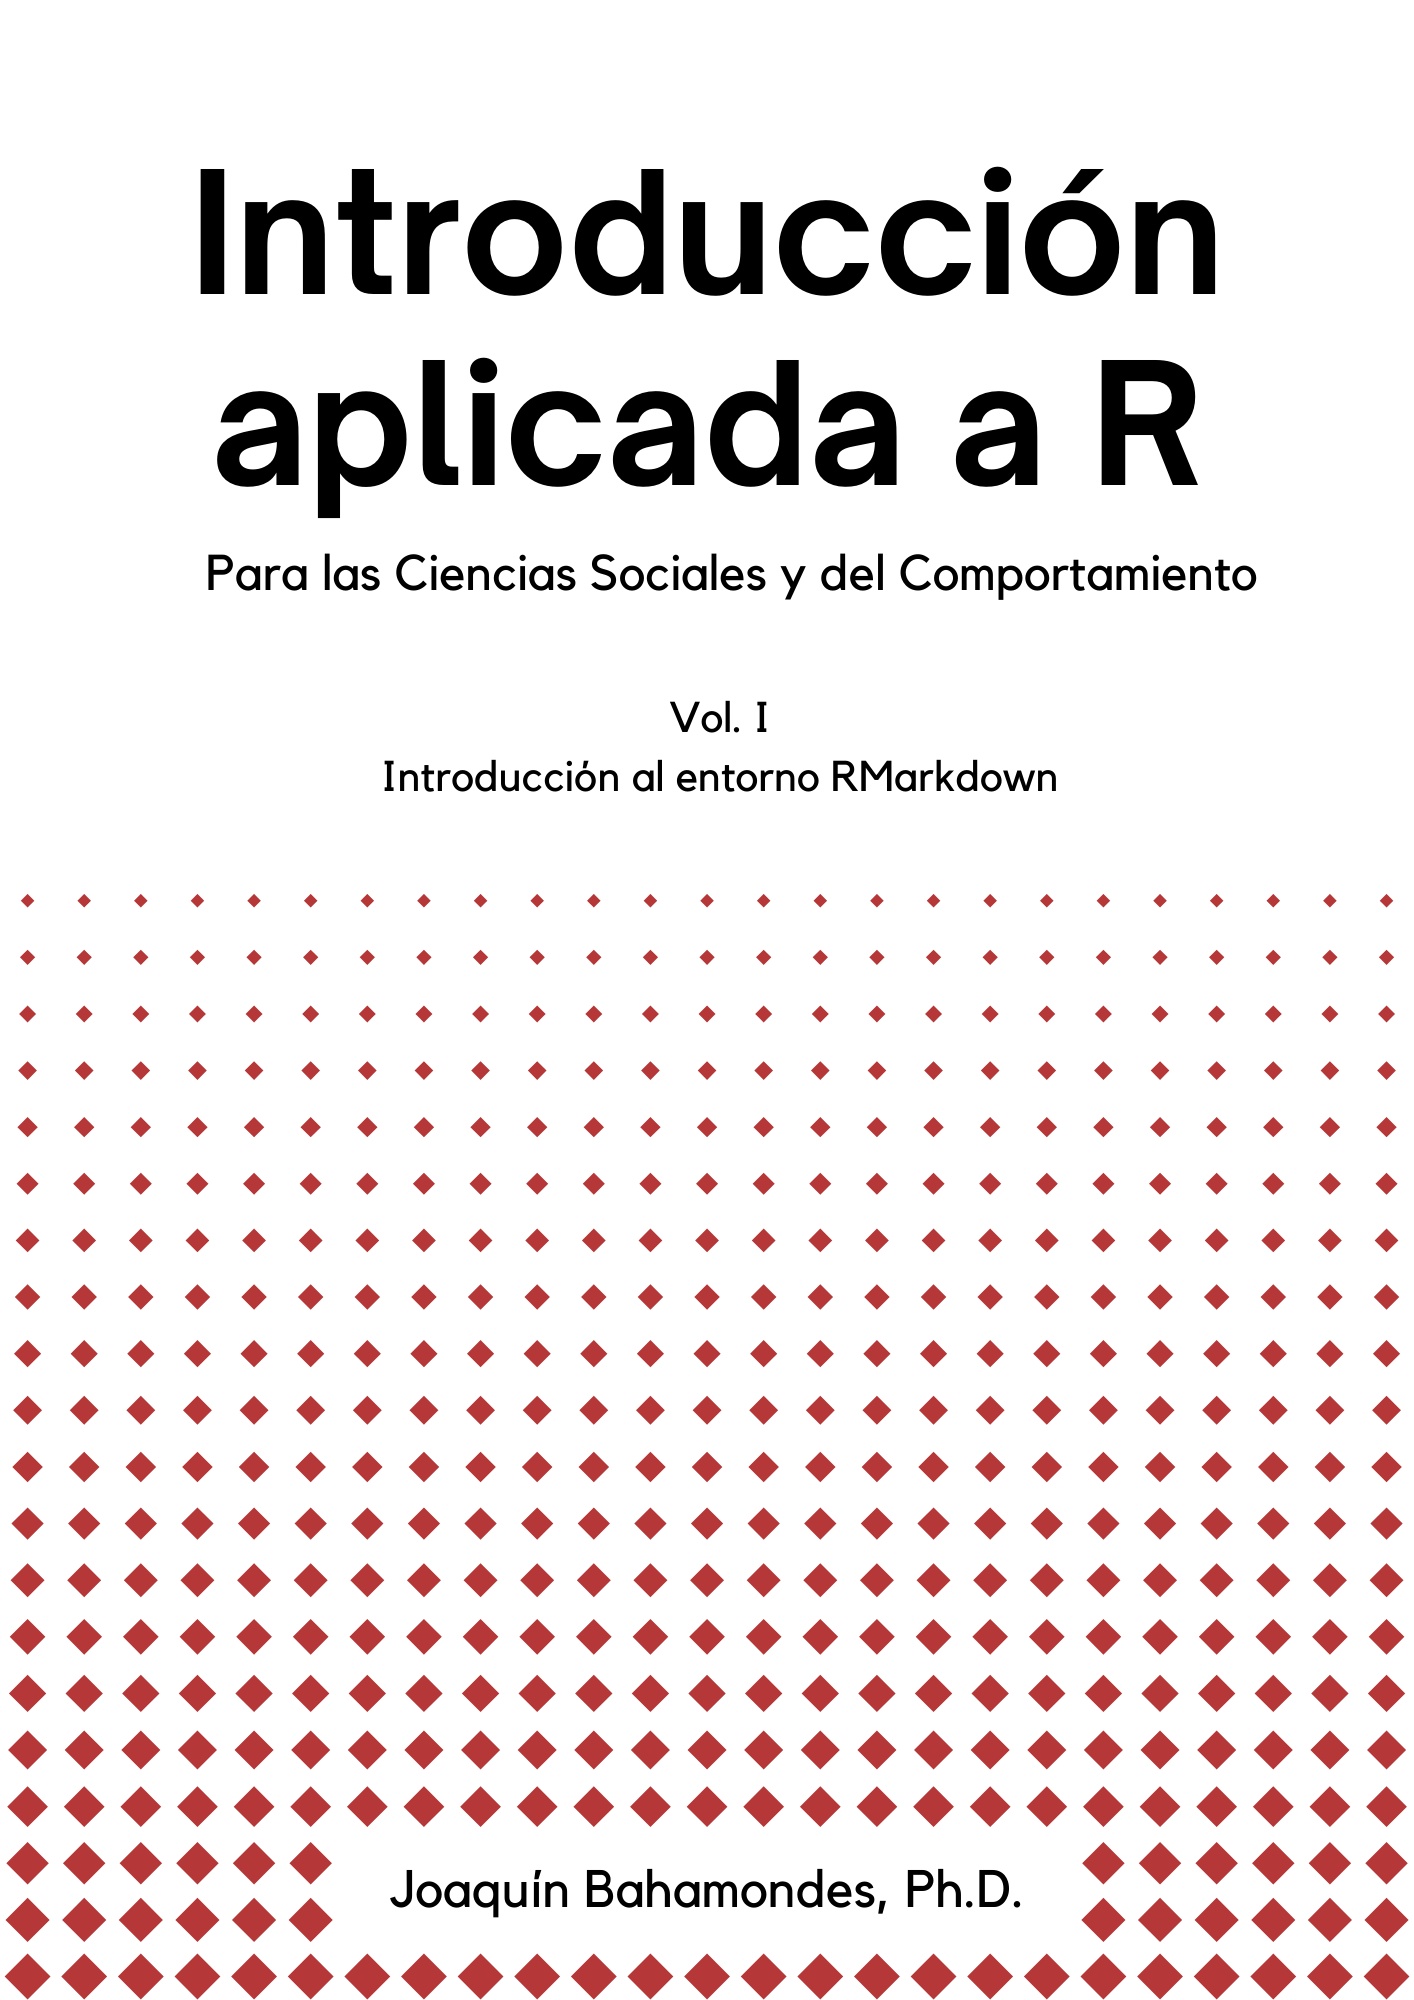
\includegraphics[width=4.16667in,height=\textheight]{_bookdown_files/images/1.png}

El presente documento tiene como objetivo introducir el uso de R, bajo criterios de \href{https://es.wikipedia.org/wiki/Ciencia_abierta}{\textbf{ciencia abierta}}, para el ordenamiento y ejecución de código aplicado principalmente a las ciencias sociales y del comportamiento. Por lo tanto, este documento no es un libro de estadística, sino una guía técnica, específica para el uso de R en \href{https://posit.co/download/rstudio-desktop/}{\textbf{RStudio}} y la implementación de su código.

Este volumen, en particular, presenta algunos de los fundamentos del uso de R, sugerencias para el ordenamiento del código, uso de notación básica y funciones esenciales.

Cualquier duda, comentario o sugerencia, por favor dirigirla a Joaquín Bahamondes, autor de esta guía, al e-mail \href{mailto:jbahamondes@ucn.cl}{\nolinkurl{jbahamondes@ucn.cl}}

\hypertarget{por-quuxe9-r}{%
\section*{¿Por qué R?}\label{por-quuxe9-r}}
\addcontentsline{toc}{section}{¿Por qué R?}

El programa R es una consola de análisis de operadores lógicos, principalmente diseñado para análisis estadísticos, con su propio lenguaje de programación. Quizás más importante, es un software de código abierto, gratuito, de gran flexibilidad y capacidad para gestionar distintos tipos de información y producir múltiples resultados, desde output de análisis estadístico, hasta imágenes, archivos de texto y sitios web (entre otros).

\hypertarget{uxedndice}{%
\section*{Índice}\label{uxedndice}}
\addcontentsline{toc}{section}{Índice}

\begin{enumerate}
\def\labelenumi{\arabic{enumi}.}
\tightlist
\item
  \protect\hyperlink{estructura-flujo}{Estructura y flujo de trabajo en R}\\
\item
  \protect\hyperlink{notacion-funciones}{Notación y funciones básicas}\\
\item
  \protect\hyperlink{paquetes}{Cargar paquetes}\\
\item
  \protect\hyperlink{simulaciuxf3n}{Simulación simple de datos}\\
\item
  \protect\hyperlink{carga-datos}{Cargar datos}
\end{enumerate}

\hypertarget{estructura-flujo}{%
\chapter{Estructura y flujo de trabajo}\label{estructura-flujo}}

Como punto de partida, es preciso comprender la organización del código en el espacio de trabajo de R. En esta sección, nos referiremos a la estructura recomendada para organizar el entorno de trabajo (i.e., las carpetas y el flujo entre ellas), así como algunas recomendaciones generales respecto de la estructura interna de cada documento de trabajo.

\hypertarget{flujo-de-trabajo-ipo}{%
\section{Flujo de trabajo IPO}\label{flujo-de-trabajo-ipo}}

El modelo input--process--output (IPO) es una forma ampliamente adoptada en análisis de sistemas y procesamiento de datos, con el objetivo de proveer un ordenamiento eficiente de la información y los procesos implicados en algún proyecto. Para nuestros propósitos, el protocolo IPO es una forma de ordenar la estructura y el flujo de las carpetas de un proyecto R (\href{https://support.posit.co/hc/en-us/articles/200526207-Using-RStudio-Projects}{R project file}) vinculado a un (o una serie de) estudio(s). Éste es enfáticamente recomendado por el Laboratorio de Ciencia Social Abierta (LISA), dado que es altamente adecuado para la apertura de los materiales en base a criterios de Ciencia Abierta.

La implementación de la reproducibilidad en este tipo de protocolos se basa en generar un conjunto de archivos auto-contenidos, organizados bajo una estructura de proyecto, que cualquier persona pueda acceder y usar. En otras palabras, debe tener todo lo que necesita para ejecutar, y volver a ejecutar el análisis, obteniendo los mismos productos.

Específicamente, el protocolo \textbf{IPO}, para flujo de investigación reproducible, se refiere a Input-Procesamiento-Output. Esta organización permite estructurar los archivos en tres carpetas.\\
El directorio correspondiente al \textbf{input} contiene todo aquello que ``alimentaremos'' a los procesos. Se trata de archivos de \emph{etrada}, que no modificaremos en su archivo original, pero cuya información resulta relevante para los procedimientos a desarrollar. Algunos ejemplos son archivos de datos en bruto, imágenes, etc.\\
Una segunda carpeta contiene los archivos de \textbf{proceso}, usualmente \texttt{.rmd}. Estos corresponden a aquellos donde guardamos el código que ejecuta operaciones sobre los inputs. Por ejemplo, aquí guardaríamos nuestros códigos de gestión de datos o de análisis estadístico.\\
Finalmente, la última carpeta corresponde al \textbf{output}, es decir, las \emph{salidas}. Aquí se alojan los resultados de los procesos, como versiones limpias o modificadas de los datos, o las imágenes (e.g., gráficos) derivados de los archivos de proceso. Si bien estos productos pueden ser utilizados como entradas por algún archivo de proceso, es importante distinguirlos de aquellos que corresponden a archivos en bruto, alojados en la carpeta input, dado que todo output es el resultado de algún proceso llevado a cabo por nosotro/as en el entorno de nuestro proyecto.

El siguiente diagrama grafica la estructura general de estas carpetas:

\begin{Shaded}
\begin{Highlighting}[]
\NormalTok{├── input}\SpecialCharTok{:}\NormalTok{ información externa como datos, imágenes, .bib}\SpecialCharTok{:}  
\NormalTok{│   ├── data}\SpecialCharTok{:}
\NormalTok{│     ├── original }\SpecialCharTok{:}\NormalTok{ archivos de datos originales y metadatos disponibles}
\NormalTok{│     ├── proc     }\SpecialCharTok{:}\NormalTok{ archivos de datos procesados}
\NormalTok{│   ├── imagenes}
\NormalTok{│   ├── bib}\SpecialCharTok{:}\NormalTok{ archivos de bibliografía}
\NormalTok{│   ├── prereg}\SpecialCharTok{:}\NormalTok{ archivos de pre}\SpecialCharTok{{-}}\NormalTok{registro si están disponibles}
\SpecialCharTok{|}
\NormalTok{├── procesamiento}\SpecialCharTok{:}
\NormalTok{│   }\SpecialCharTok{{-}}\NormalTok{ preparacion.Rmd}
\NormalTok{│   }\SpecialCharTok{{-}}\NormalTok{ analisis.Rmd}
\NormalTok{│}
\NormalTok{├── output}\SpecialCharTok{:}\NormalTok{ tablas, gráficos y otras salidas del procesamiento.}
\NormalTok{│   ├── gráficos}
\NormalTok{│   ├── tablas}
\NormalTok{│}
\SpecialCharTok{{-}}\NormalTok{ readme.md }\SpecialCharTok{:}\NormalTok{ archivo general de introducción}
\SpecialCharTok{{-}}\NormalTok{ paper.md o paper.Rmd }\SpecialCharTok{/}\NormalTok{ paper.html }\SpecialCharTok{/}\NormalTok{ paper.pdf}\SpecialCharTok{:}\NormalTok{ el artículo}\SpecialCharTok{/}\NormalTok{paper}
\end{Highlighting}
\end{Shaded}

Obtenido desde \url{https://lisa-coes.netlify.app/ipo-repro/}

\hypertarget{estructura-de-un-documento-rmarkdown}{%
\section{Estructura de un documento Rmarkdown}\label{estructura-de-un-documento-rmarkdown}}

Las secciones de un documento de R, cualquiera sea (archivo de sólo código, RMarkdown o un proyecto) pueden ser organizadas bajo distintos niveles de títulos, los que anidan el contenido correspondiente. Como regla general, debe haber sólo un título de nivel uno (\texttt{\#}) por archivo \texttt{.rmd}, y pueden haber múltiples subtítulos de nivel dos (\texttt{\#\#}), tres (\texttt{\#\#\#}), o de mayor subordinación (\texttt{\#\#\#\#...}).
En Rmarkdown, bajo cada título o subtítulos, pueden incluirse párrafos de texto como este, lo que no constituye material ejecutable, de modo que éste no será analizado de ninguna forma por el programa, sólo será presentado.

Toda vez que queramos incluir código ejecutable para procesar algún tipo de información en Rmarkdown, debemos usar \texttt{chunks}. Los \texttt{chunks} son bloques de código ejecutable, los que R entenderá como contenedores de material analizable. En Rmarkdown, se puede crear rápidamente un chunk con el atajo \textbf{ctrl + Alt + i}. Verá inmediatamente un bloque de código tal como el que se presenta a continuación:

\begin{Shaded}
\begin{Highlighting}[]
\StringTok{\textasciigrave{}\textasciigrave{}\textasciigrave{}}\AttributeTok{\{r\}}
\AttributeTok{\# Esto es un comentario dentro de un chunk. Recuerde que esto será omitido.}
\AttributeTok{\# La siguiente operación será ejecutada.}

\AttributeTok{5+2 }

\StringTok{\textasciigrave{}\textasciigrave{}\textasciigrave{}}
\end{Highlighting}
\end{Shaded}

\hypertarget{notacion-funciones}{%
\chapter{Notación y Funciones básicas}\label{notacion-funciones}}

\hypertarget{notaciuxf3n-esencial}{%
\section{Notación esencial}\label{notaciuxf3n-esencial}}

En R, los operadores básicos son:

\begin{longtable}[]{@{}ll@{}}
\toprule\noalign{}
Notación/función & símbolo usado \\
\midrule\noalign{}
\endhead
\bottomrule\noalign{}
\endlastfoot
\protect\hyperlink{asignaciuxf3n}{Asignación} & \textless- \\
\protect\hyperlink{comentario}{Comentario} & \# \\
\protect\hyperlink{combinar}{Combinar} & c() \\
\protect\hyperlink{separador}{Separador de Argumentos} & , \\
\protect\hyperlink{texto}{Texto} & ``\,'' o '\,' \\
\protect\hyperlink{equivalencia}{Equivalencia} & == \\
\protect\hyperlink{OR}{Operador O} & \textbar{} \\
\protect\hyperlink{comparaciuxf3n}{Comparación} & \textgreater, \textless, \textgreater=, \textless= \\
\protect\hyperlink{acceso}{Acceso a columnas de dato, matriz o lista} & \$ \\
\protect\hyperlink{indexaciuxf3n}{Indexación} & {[}{]} \\
\protect\hyperlink{llamada}{Llamada de función o agrupación} & () \\
\protect\hyperlink{pertenencia}{Pertenencia} & \%in\% \\
\protect\hyperlink{negaciuxf3n}{Negación} & ! \\
\protect\hyperlink{secuencia}{Secuencia} & : \\
\protect\hyperlink{aritmeticos}{Operadores aritméticos} & *, /, +, - \\
\end{longtable}

\hypertarget{asignaciuxf3n}{%
\subsection{\textless- (Asignación)}\label{asignaciuxf3n}}

Uso: Asigna valores a una variable. También se puede usar = para asignaciones básicas, pero \textless- es el operador recomendado.\\
Ejemplo:

\begin{Shaded}
\begin{Highlighting}[]
\NormalTok{x }\OtherTok{\textless{}{-}} \DecValTok{10}
\NormalTok{y }\OtherTok{\textless{}{-}} \StringTok{"texto"}
\end{Highlighting}
\end{Shaded}

Nota: -\textgreater{} también existe, aunque es poco común y asigna en la dirección opuesta (valor -\textgreater{} variable).

\hypertarget{comentario}{%
\subsection{\# (Comentario)}\label{comentario}}

Uso: Agrega comentarios en el código. R ignora todo el texto a la derecha del \# en esa línea.\\
Ejemplo:

\begin{Shaded}
\begin{Highlighting}[]
\NormalTok{x }\OtherTok{\textless{}{-}} \DecValTok{10}  \CommentTok{\# Este es un comentario}
\end{Highlighting}
\end{Shaded}

\hypertarget{combinar}{%
\subsection{c (Combinar)}\label{combinar}}

Uso: Agrupa distintos elementos en un listado o grupo que puede utilizarse como bloque para múltiples propósitos.\\
Ejemplo:

\begin{Shaded}
\begin{Highlighting}[]
\NormalTok{sujeto01 }\OtherTok{\textless{}{-}} \FunctionTok{c}\NormalTok{(x,y)  }\CommentTok{\# agrupa respuestas de un sujeto}
\NormalTok{sujeto02 }\OtherTok{\textless{}{-}} \FunctionTok{c}\NormalTok{(}\DecValTok{5}\NormalTok{, }\StringTok{"texto 2"}\NormalTok{) }\CommentTok{\# lo mismo para sujeto 2}
\end{Highlighting}
\end{Shaded}

Nota: Los comentarios son esenciales para documentar y hacer el código más comprensible.

\hypertarget{separador}{%
\subsection{, (Separador de Argumentos)}\label{separador}}

Uso: Separa elementos en funciones o elementos de un vector/matriz.\\
Ejemplo:

\begin{Shaded}
\begin{Highlighting}[]
\FunctionTok{c}\NormalTok{(}\DecValTok{1}\NormalTok{, }\DecValTok{2}\NormalTok{, }\DecValTok{3}\NormalTok{)  }\CommentTok{\# Crea un vector con 3 elementos}
\end{Highlighting}
\end{Shaded}

Nota: También se usa para separar filas y columnas en indexación de matrices y data frames.

\hypertarget{texto}{%
\subsection{``\,'' o '\,' (Definición de Cadenas de Texto)}\label{texto}}

Uso: Define valores de tipo carácter (strings).
Ejemplo:

\begin{Shaded}
\begin{Highlighting}[]
\NormalTok{nombre }\OtherTok{\textless{}{-}} \StringTok{"Joaquín"}
\NormalTok{apellido }\OtherTok{\textless{}{-}} \StringTok{\textquotesingle{}Bahamondes\textquotesingle{}}
\end{Highlighting}
\end{Shaded}

Nota: En R, '' y ' son equivalentes. Sin embargo, es más común usar '' para cadenas de texto.

\hypertarget{equivalencia}{%
\subsection{== (Igualdad Lógica)}\label{equivalencia}}

Uso: Compara si dos valores son iguales. Devuelve TRUE o FALSE.\\
Ejemplo:

\begin{Shaded}
\begin{Highlighting}[]
\NormalTok{x }\OtherTok{\textless{}{-}} \DecValTok{5}
\NormalTok{y }\OtherTok{\textless{}{-}} \DecValTok{5}
\NormalTok{x }\SpecialCharTok{==}\NormalTok{ y  }\CommentTok{\# TRUE}
\end{Highlighting}
\end{Shaded}

Nota: No confundir con = que es un operador de asignación (aunque puede ser usado en argumentos de funciones).

\hypertarget{OR}{%
\subsection{\textbar{} (OR Lógico)}\label{OR}}

Uso: Devuelve TRUE si al menos una de las condiciones es TRUE.
Ejemplo:

\begin{Shaded}
\begin{Highlighting}[]
\NormalTok{(x }\SpecialCharTok{==} \DecValTok{5}\NormalTok{) }\SpecialCharTok{|}\NormalTok{ (y }\SpecialCharTok{==} \DecValTok{10}\NormalTok{)}
\end{Highlighting}
\end{Shaded}

\hypertarget{comparaciuxf3n}{%
\subsection{\textgreater, \textless, \textgreater=, \textless= (Comparación)}\label{comparaciuxf3n}}

Uso: Operadores de comparación para verificar si un valor es mayor, menor, mayor o igual, o menor o igual que otro.
Ejemplo:

\begin{Shaded}
\begin{Highlighting}[]
\NormalTok{x }\SpecialCharTok{\textgreater{}} \DecValTok{3}   \CommentTok{\# TRUE si x es mayor que 3}
\end{Highlighting}
\end{Shaded}

\begin{verbatim}
## [1] TRUE
\end{verbatim}

\begin{Shaded}
\begin{Highlighting}[]
\NormalTok{y }\SpecialCharTok{\textless{}=} \DecValTok{10} \CommentTok{\# TRUE si y es menor o igual a 10}
\end{Highlighting}
\end{Shaded}

\begin{verbatim}
## [1] FALSE
\end{verbatim}

\hypertarget{acceso}{%
\subsection{\$ (Acceso a Columnas de Data Frames o Listas)}\label{acceso}}

Uso: Permite acceder a una columna específica en un data frame o a un elemento en una lista.
Ejemplo:

\begin{Shaded}
\begin{Highlighting}[]
\NormalTok{df }\OtherTok{\textless{}{-}} \FunctionTok{data.frame}\NormalTok{(}\AttributeTok{a =} \DecValTok{1}\SpecialCharTok{:}\DecValTok{3}\NormalTok{, }\AttributeTok{b =} \DecValTok{4}\SpecialCharTok{:}\DecValTok{6}\NormalTok{)}
\NormalTok{df}\SpecialCharTok{$}\NormalTok{a  }\CommentTok{\# Devuelve la columna \textquotesingle{}a\textquotesingle{}}
\end{Highlighting}
\end{Shaded}

\begin{verbatim}
## [1] 1 2 3
\end{verbatim}

Nota: Es especialmente útil en análisis de datos cuando necesitas acceder rápidamente a columnas (i.e., variables) específicas.

\hypertarget{indexaciuxf3n}{%
\subsection{{[}{]} (Indexación)}\label{indexaciuxf3n}}

Uso: Extrae elementos de vectores, listas, matrices o data frames.
Ejemplo:

\begin{Shaded}
\begin{Highlighting}[]
\NormalTok{vec }\OtherTok{\textless{}{-}} \FunctionTok{c}\NormalTok{(}\DecValTok{10}\NormalTok{, }\DecValTok{20}\NormalTok{, }\DecValTok{30}\NormalTok{)}
\NormalTok{vec[}\DecValTok{1}\NormalTok{]  }\CommentTok{\# Devuelve el primer elemento}
\end{Highlighting}
\end{Shaded}

\begin{verbatim}
## [1] 10
\end{verbatim}

Nota: {[}fila, columna{]} se usa para acceder a elementos en matrices o data frames.

\hypertarget{llamada}{%
\subsection{() (Llamada de Funciones o Agrupación)}\label{llamada}}

Uso: Agrupa expresiones o se usa para pasar argumentos en funciones. Hemos estado usándola para aplicar todas las funciones presentadas anteriormente.
Ejemplo:

\begin{Shaded}
\begin{Highlighting}[]
\NormalTok{suma }\OtherTok{\textless{}{-}} \FunctionTok{sum}\NormalTok{(}\DecValTok{1}\NormalTok{, }\DecValTok{2}\NormalTok{, }\DecValTok{3}\NormalTok{)  }\CommentTok{\# Llama a la función sum con tres argumentos}
\end{Highlighting}
\end{Shaded}

Nota: También se usa para forzar el orden de operaciones en expresiones matemáticas.

\hypertarget{pertenencia}{%
\subsection{\%in\% (Pertenencia)}\label{pertenencia}}

Uso: Verifica si un elemento está presente en un vector.
Ejemplo:

\begin{Shaded}
\begin{Highlighting}[]
\NormalTok{x }\OtherTok{\textless{}{-}} \DecValTok{5}
\NormalTok{x }\SpecialCharTok{\%in\%} \FunctionTok{c}\NormalTok{(}\DecValTok{1}\NormalTok{, }\DecValTok{2}\NormalTok{, }\DecValTok{3}\NormalTok{, }\DecValTok{5}\NormalTok{)  }\CommentTok{\# TRUE}
\end{Highlighting}
\end{Shaded}

\begin{verbatim}
## [1] TRUE
\end{verbatim}

\hypertarget{negaciuxf3n}{%
\subsection{! (Negación)}\label{negaciuxf3n}}

Uso: Niega una condición lógica (convierte TRUE a FALSE y viceversa).
Ejemplo:

\begin{Shaded}
\begin{Highlighting}[]
\NormalTok{x }\OtherTok{\textless{}{-}} \ConstantTok{FALSE}
\SpecialCharTok{!}\NormalTok{x  }\CommentTok{\# TRUE}
\end{Highlighting}
\end{Shaded}

\begin{verbatim}
## [1] TRUE
\end{verbatim}

\hypertarget{secuencia}{%
\subsection{: (Secuencia)}\label{secuencia}}

Uso: Genera una secuencia de números enteros.
Ejemplo:

\begin{Shaded}
\begin{Highlighting}[]
\DecValTok{1}\SpecialCharTok{:}\DecValTok{5}  \CommentTok{\# Genera el vector c(1, 2, 3, 4, 5)}
\end{Highlighting}
\end{Shaded}

\begin{verbatim}
## [1] 1 2 3 4 5
\end{verbatim}

\hypertarget{operadores-aritmuxe9ticos-aritmeticos}{%
\subsection{*, /, +, - (Operadores Aritméticos) \{\#aritmeticos\}}\label{operadores-aritmuxe9ticos-aritmeticos}}

Uso: Realizan operaciones aritméticas básicas de multiplicación, división, suma y resta.
Ejemplo:
r
Copiar código
x \textless- 10
y \textless- 5
x + y \# Suma, devuelve 15
x * y \# Multiplicación, devuelve 50

En esta sección, se detallan las funciones básicas más comunes que necesitaremos aplicar al analizar datos en R.\\
En general, el lenguaje R se trata de aplicar funciones a objetos, de modo que ``abrazamos'' un objeto \(x\) con una función para obtener un resultado deseado, en el formato \texttt{función(x)}. El objeto \(x\) puede tomar múltiples formas, desde una base de datos, un listado de palabras, o un número único.

Probablemente la función más útil en R es \texttt{combine}, la cual se aplica simplemente con \texttt{c(x)}. consideremos el siguiente ejemplo:

\hypertarget{combine}{%
\subsection{Combine}\label{combine}}

Esta función sirve, entre otras cosas, para combinar distintos elementos (e.g., valores) dentro de una misma lista. Por ejemplo, si tenemos 5 sujetos cuyas edades son 28, 37, 29, 43, y 34, podemos crear un objeto (en este caso, un vector) que contenga dicha información, simplemente con el siguiente código

\begin{Shaded}
\begin{Highlighting}[]
\NormalTok{edades }\OtherTok{\textless{}{-}} \FunctionTok{c}\NormalTok{(}\DecValTok{28}\NormalTok{, }\DecValTok{37}\NormalTok{, }\DecValTok{29}\NormalTok{, }\DecValTok{43}\NormalTok{, }\DecValTok{34}\NormalTok{)}
\end{Highlighting}
\end{Shaded}

Al ejecutar ese código, se creará un nuevo objeto, llamado \texttt{edades}, que contiene los 5 valores. Por lo tanto, dado que el objeto corresponde a una lista de números, podemos aplicar funciones algebráicas, tal como calcular la media \texttt{mean(x)}, o la desviación típica \texttt{sd(x)}, para lo cual obtendremos:

\texttt{mean(edades)} = 34.2\\
\texttt{sd(edades)} = 6.14

\hypertarget{paquetes}{%
\chapter{Instalación y uso de paquetes}\label{paquetes}}

En R, los paquetes son colecciones organizadas de funciones, datos y/o documentación diseñadas para facilitar tareas específicas en programación y análisis. Lo principal es que extienden las capacidades base de R, permitiendo a los usuarios acceder a funcionalidades adicionales sin tener que programarlas desde cero.

\hypertarget{instalaciuxf3n}{%
\section{Instalación:}\label{instalaciuxf3n}}

Los paquetes deben instalarse una vez antes de su primer uso en el entorno de R. Esto se hace con la función

\begin{Shaded}
\begin{Highlighting}[]
\FunctionTok{install.packages}\NormalTok{(}\StringTok{"nombre{-}del{-}paquete"}\NormalTok{)}
\end{Highlighting}
\end{Shaded}

la cual descarga el paquete y lo guarda en la biblioteca de R local.

\hypertarget{carga}{%
\section{Carga:}\label{carga}}

Después de instalar un paquete, se debe cargar en cada nueva sesión de R para acceder a sus funciones, lo cual se hace usando

\begin{Shaded}
\begin{Highlighting}[]
\FunctionTok{library}\NormalTok{(nombre\_del\_paquete)}
\end{Highlighting}
\end{Shaded}

Esto permite que R reconozca las funciones y datos contenidos en el paquete.

\hypertarget{uso}{%
\section{Uso:}\label{uso}}

Una vez cargado, el usuario puede llamar a las funciones y utilizar los datos incluidos en el paquete de manera inmediata. Las funciones dentro del paquete están diseñadas para integrarse con el entorno R y suelen seguir la misma sintaxis y estilo.

\hypertarget{actualizaciuxf3n-y-gestiuxf3n}{%
\section{Actualización y Gestión:}\label{actualizaciuxf3n-y-gestiuxf3n}}

Los paquetes deben actualizarse periódicamente para aprovechar mejoras, correcciones y nuevas funcionalidades. Esto se hace con

\begin{Shaded}
\begin{Highlighting}[]
\FunctionTok{update.packages}\NormalTok{()}
\end{Highlighting}
\end{Shaded}

\hypertarget{uso-de-pacman}{%
\section{Uso de Pacman}\label{uso-de-pacman}}

\textbf{Pacman} es un paquete destinado a facilitar la instalación y carga de paquetes en R.\\
En esta guía, recomendamos hacer uso rutinario de la función \texttt{p\_load}, dentro de la cual se puede definir un conjunto de paquetes (seprados por ,) que deban cargarse, según las funciones necesarias para la sesión. Una de las principales utilidades de esta función es que instala aquellos paquetes que no estén instalados en el entorno local.

\begin{Shaded}
\begin{Highlighting}[]
\NormalTok{pacman}\SpecialCharTok{::}\FunctionTok{p\_load}\NormalTok{()}
\end{Highlighting}
\end{Shaded}

\hypertarget{simulaciuxf3n}{%
\chapter{Simulación}\label{simulaciuxf3n}}

Simular datos en R es una técnica útil para pruebas, experimentos o validaciones estadísticas sin necesidad de datos reales. Con funciones como \texttt{rnorm()}, \texttt{runif()}, \texttt{sample()}, y \texttt{rbinom()}, R permite generar datos que cumplen con ciertas distribuciones y características básicas, como la media, la desviación estándar, la cantidad de observaciones, entre otras.

\hypertarget{generaciuxf3n-de-datos}{%
\section{Generación de Datos}\label{generaciuxf3n-de-datos}}

\hypertarget{datos-normales}{%
\subsection{Datos Normales:}\label{datos-normales}}

Para generar datos con una distribución normal, se usa \texttt{rnorm(n,\ mean,\ sd)}, donde:

\begin{itemize}
\tightlist
\item
  \texttt{n} es el número de observaciones,\\
\item
  \texttt{mean} es la media,\\
\item
  \texttt{sd} es la desviación estándar.
\end{itemize}

\begin{Shaded}
\begin{Highlighting}[]
\NormalTok{datos\_normales }\OtherTok{\textless{}{-}} \FunctionTok{rnorm}\NormalTok{(}\DecValTok{1000}\NormalTok{, }\AttributeTok{mean =} \FloatTok{3.8}\NormalTok{, }\AttributeTok{sd =} \FloatTok{1.1}\NormalTok{)}
\CommentTok{\# Imponer límites mínimo y máximo}
\NormalTok{minimo }\OtherTok{\textless{}{-}} \DecValTok{1}
\NormalTok{maximo }\OtherTok{\textless{}{-}} \DecValTok{7}
\NormalTok{datos\_normales\_lim }\OtherTok{\textless{}{-}} \FunctionTok{ifelse}\NormalTok{(datos\_normales }\SpecialCharTok{\textless{}}\NormalTok{ minimo, minimo, }
                         \FunctionTok{ifelse}\NormalTok{(datos\_normales }\SpecialCharTok{\textgreater{}}\NormalTok{ maximo, maximo, datos\_normales))}

\FunctionTok{hist}\NormalTok{(datos\_normales\_lim, }
     \AttributeTok{breaks =} \DecValTok{7}\NormalTok{, }
     \AttributeTok{col =} \StringTok{"lightyellow"}\NormalTok{, }
     \AttributeTok{main =} \StringTok{"Distribución Normal"}\NormalTok{, }
     \AttributeTok{xlab =} \StringTok{"Valores"}\NormalTok{,}
     \AttributeTok{ylab =} \StringTok{"Frecuencia"}\NormalTok{)}
\end{Highlighting}
\end{Shaded}

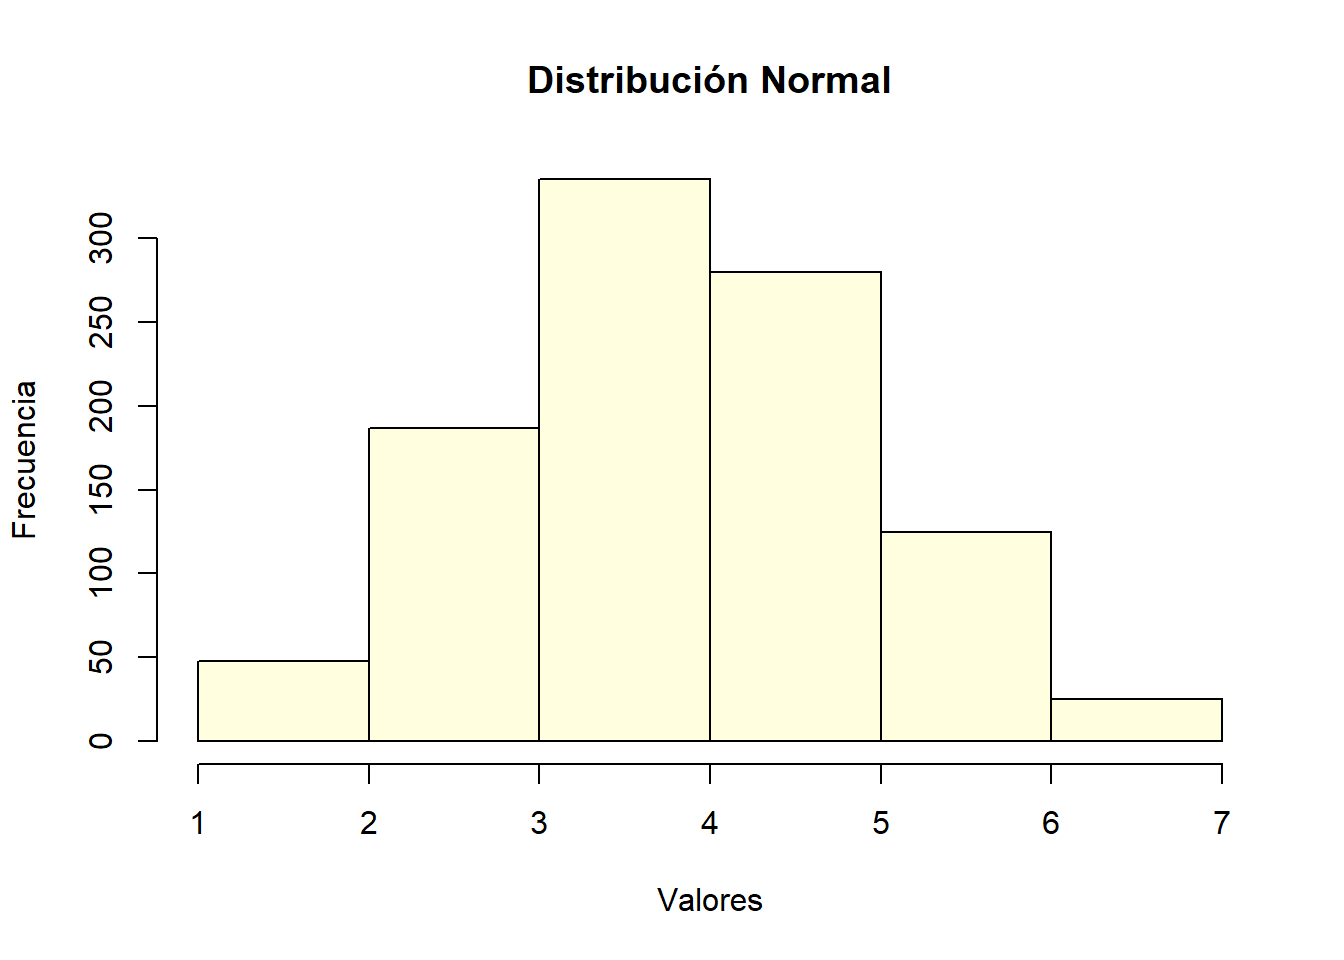
\includegraphics{_main_files/figure-latex/unnamed-chunk-23-1.pdf}

\hypertarget{datos-uniformes}{%
\subsection{Datos Uniformes:}\label{datos-uniformes}}

Para una distribución uniforme, que genera valores entre un rango específico con la misma probabilidad, se usa \texttt{runif(n,\ min,\ max)}:

\begin{itemize}
\tightlist
\item
  \texttt{n} es el número de observaciones,\\
\item
  \texttt{min} y \texttt{max} definen el rango.
\end{itemize}

\begin{Shaded}
\begin{Highlighting}[]
\NormalTok{datos\_uniformes }\OtherTok{\textless{}{-}} \FunctionTok{runif}\NormalTok{(}\DecValTok{100}\NormalTok{, }\AttributeTok{min =} \DecValTok{1}\NormalTok{, }\AttributeTok{max =} \DecValTok{7}\NormalTok{)}
\FunctionTok{hist}\NormalTok{(datos\_uniformes, }
     \AttributeTok{breaks =} \DecValTok{7}\NormalTok{, }
     \AttributeTok{col =} \StringTok{"lightyellow"}\NormalTok{, }
     \AttributeTok{main =} \StringTok{"Distribución Uniforme"}\NormalTok{, }
     \AttributeTok{xlab =} \StringTok{"Valores"}\NormalTok{,}
     \AttributeTok{ylab =} \StringTok{"Frecuencia"}\NormalTok{)}
\end{Highlighting}
\end{Shaded}

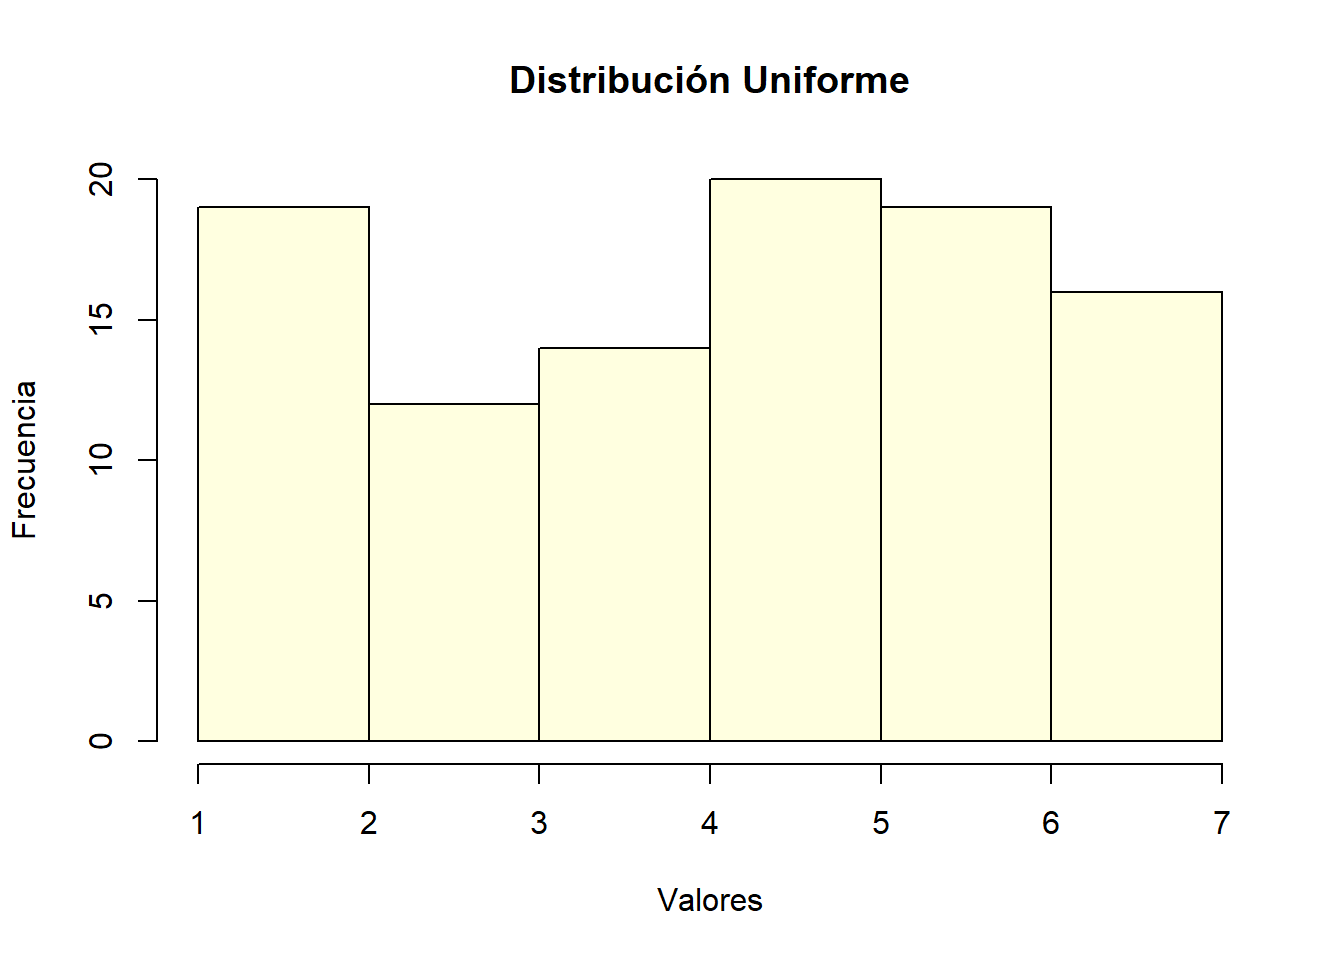
\includegraphics{_main_files/figure-latex/unnamed-chunk-24-1.pdf}

\hypertarget{datos-binomiales}{%
\subsection{Datos Binomiales:}\label{datos-binomiales}}

Para datos binarios o con un número fijo de éxitos (p.ej., tiradas de moneda), se usa \texttt{rbinom(n,\ size,\ prob)}, donde:

\begin{itemize}
\tightlist
\item
  \texttt{n} es el número de observaciones,\\
\item
  \texttt{size} es el número de ensayos,\\
\item
  \texttt{prob} es la probabilidad de éxito en cada ensayo.
\end{itemize}

\begin{Shaded}
\begin{Highlighting}[]
\NormalTok{datos\_binomiales }\OtherTok{\textless{}{-}} \FunctionTok{rbinom}\NormalTok{(}\DecValTok{100}\NormalTok{, }\AttributeTok{size =} \DecValTok{1}\NormalTok{, }\AttributeTok{prob =} \FloatTok{0.5}\NormalTok{)}
\FunctionTok{hist}\NormalTok{(datos\_binomiales, }
     \AttributeTok{breaks =} \DecValTok{12}\NormalTok{,}
     \AttributeTok{col =} \StringTok{"lightyellow"}\NormalTok{, }
     \AttributeTok{main =} \StringTok{"Distribución binomial"}\NormalTok{, }
     \AttributeTok{xlab =} \StringTok{"Valores"}\NormalTok{,}
     \AttributeTok{ylab =} \StringTok{"Frecuencia"}\NormalTok{)}
\end{Highlighting}
\end{Shaded}

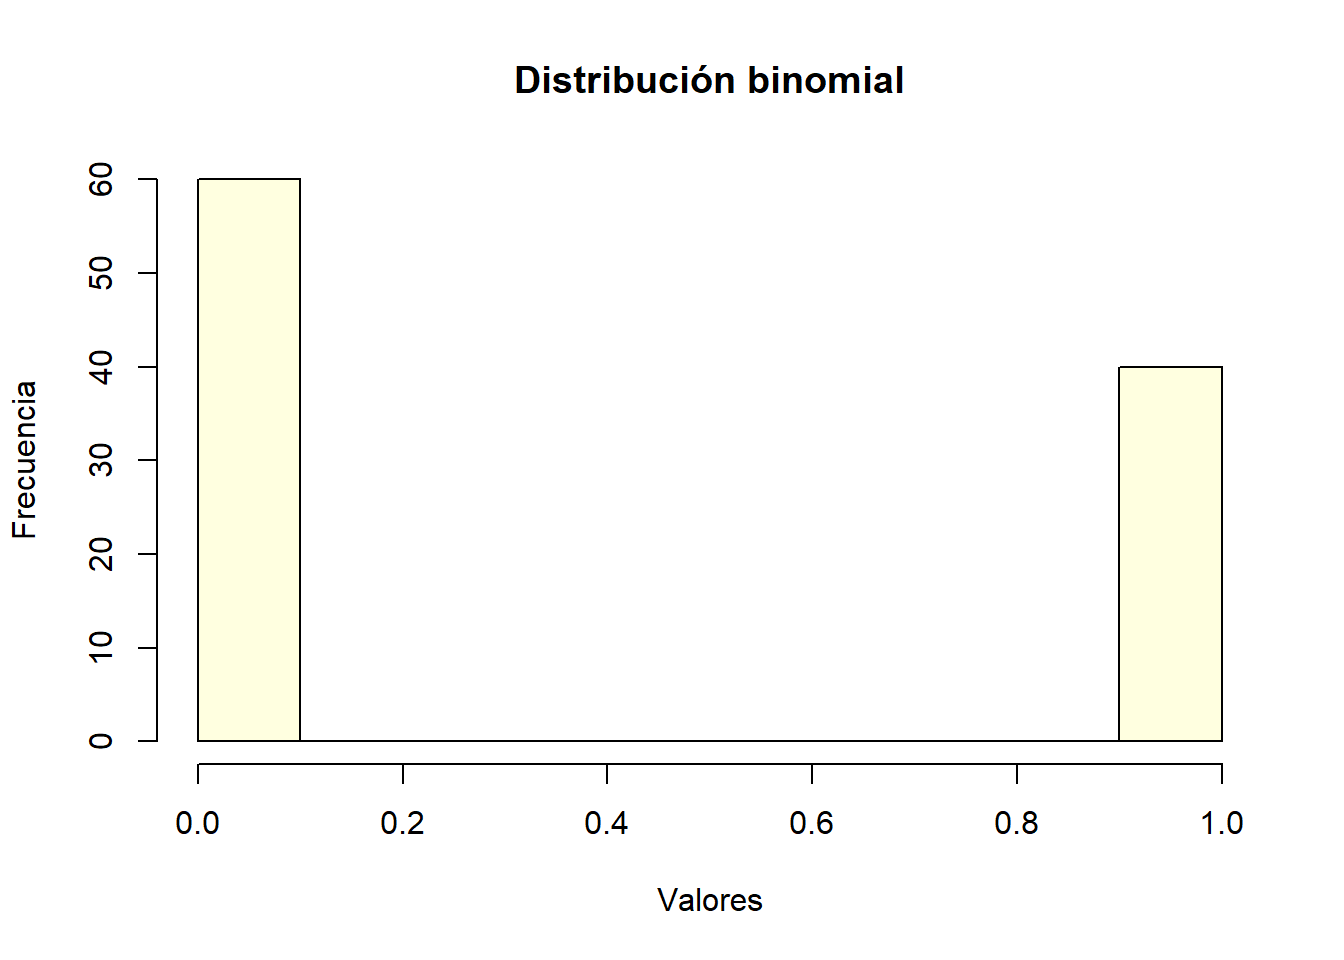
\includegraphics{_main_files/figure-latex/unnamed-chunk-25-1.pdf}

\hypertarget{manipulaciuxf3n-de-caracteruxedsticas-de-los-datos}{%
\section{Manipulación de Características de los Datos}\label{manipulaciuxf3n-de-caracteruxedsticas-de-los-datos}}

\hypertarget{cambio-de-la-media-y-desviaciuxf3n-estuxe1ndar}{%
\subsection{Cambio de la media y desviación estándar:}\label{cambio-de-la-media-y-desviaciuxf3n-estuxe1ndar}}

La media y la desviación estándar se pueden ajustar en funciones como \texttt{rnorm()} para controlar la distribución y dispersión de los datos.

\hypertarget{tamauxf1o-de-la-muestra}{%
\subsection{Tamaño de la muestra:}\label{tamauxf1o-de-la-muestra}}

Ajustando el parámetro \texttt{n}, se modifica la cantidad de datos generados, lo cual es útil para realizar pruebas de análisis en conjuntos grandes o pequeños.

\hypertarget{rango-de-valores}{%
\subsection{Rango de valores:}\label{rango-de-valores}}

Para obtener valores en rangos específicos (p.ej., entre 0 y 100), \texttt{runif()} permite definir estos límites con \texttt{min} y \texttt{max}.

Estos métodos permiten generar datos con propiedades controladas, ayudando a diseñar experimentos o pruebas que se asemejan a escenarios reales y asegurando variabilidad y control en las simulaciones.

\hypertarget{creaciuxf3n-de-una-base-de-datos-en-r}{%
\section{Creación de una base de datos en R}\label{creaciuxf3n-de-una-base-de-datos-en-r}}

A continuación, crearemos una base de dato desde cero en este mismo entorno, practicando la creación de distintos objetos, vectores, matrices, y terminando por guardar una base de datos exportable. Recuerda que las características de cualquiera de estas variables puede ser modificada a nuestro antojo, y poder ajustarlas a nuestros propósitos particulares.\\
Para no repetir sistemáticamente el mismo número en caso que queramos modificarlo, definiremos el número de casos. Para esto, simplemente guardamos en un objeto el n deseado.

\begin{Shaded}
\begin{Highlighting}[]
\NormalTok{n\_sim }\OtherTok{\textless{}{-}} \DecValTok{200}
\end{Highlighting}
\end{Shaded}

Partiremos por crear un vector identificador para un total de 200 casos. Para esto, utilizamos la función \texttt{paste()}, de modo que podamos asignar un código alfanumérico a cada fila que registre un caso.

\begin{Shaded}
\begin{Highlighting}[]
\CommentTok{\# Vector de caracteres}
\NormalTok{id\_vec }\OtherTok{\textless{}{-}} \FunctionTok{paste}\NormalTok{(}\StringTok{"id"}\NormalTok{, }\DecValTok{1}\SpecialCharTok{:}\DecValTok{200}\NormalTok{)}
\end{Highlighting}
\end{Shaded}

Ahora, inventaremos que esta muestra de 200 personas tiene edades entre los 20 a 60 años de edad. Entonces, usamos la función \texttt{sample()} para crear un listado de 200 valores aleatorios entre 20 y 60, con posibilidad de reemplazo. Como se puede observar en el código, se utilizará la función \texttt{set.seed()} para fijar la semilla que produce la aleatorización, de modo tal que no variará cada vez que ejecutemos el código, lo que permitirá la reproducibilidad.

\begin{Shaded}
\begin{Highlighting}[]
\FunctionTok{set.seed}\NormalTok{(}\DecValTok{123}\NormalTok{)  }\CommentTok{\# Para reproducibilidad}

\CommentTok{\# Vector numérico}
\NormalTok{edades }\OtherTok{\textless{}{-}} \FunctionTok{sample}\NormalTok{(}\DecValTok{20}\SpecialCharTok{:}\DecValTok{60}\NormalTok{, }\DecValTok{200}\NormalTok{, }\AttributeTok{replace =} \ConstantTok{TRUE}\NormalTok{)}
\end{Highlighting}
\end{Shaded}

Aceleremos algo el proceso, creando una matriz \texttt{matrix()} en lugar de un sólo vector. Para esto, creemos aleatoriamente 200 valores tanto para altura (en cms) como para peso (kgs).

\begin{Shaded}
\begin{Highlighting}[]
\FunctionTok{set.seed}\NormalTok{(}\DecValTok{123}\NormalTok{)}

\CommentTok{\# Matriz de altura (cm) y peso (kg)}
\NormalTok{mx\_altura\_peso }\OtherTok{\textless{}{-}} \FunctionTok{matrix}\NormalTok{(}\FunctionTok{c}\NormalTok{(}
  \FunctionTok{sample}\NormalTok{(}\DecValTok{150}\SpecialCharTok{:}\DecValTok{200}\NormalTok{, }\DecValTok{200}\NormalTok{, }\AttributeTok{replace =} \ConstantTok{TRUE}\NormalTok{),  }\CommentTok{\# Altura en cm}
  \FunctionTok{sample}\NormalTok{(}\DecValTok{50}\SpecialCharTok{:}\DecValTok{100}\NormalTok{, }\DecValTok{200}\NormalTok{, }\AttributeTok{replace =} \ConstantTok{TRUE}\NormalTok{)   }\CommentTok{\# Peso en kg}
\NormalTok{), }\AttributeTok{nrow =} \DecValTok{200}\NormalTok{, }\AttributeTok{byrow =} \ConstantTok{FALSE}\NormalTok{)}
\end{Highlighting}
\end{Shaded}

Demos nombres a las columnas (i.e., variables) usando la función \texttt{colnames()}, sobre la cual se asigna el listado de nombres, tal como si estuviésemos creando un objeto a través de una asignación \texttt{\textless{}-}. Usaremos la función \texttt{head()} para chequear que la matriz se haya dispuesto correctamente.

\begin{Shaded}
\begin{Highlighting}[]
\CommentTok{\# Asignar nombres a las columnas}
\FunctionTok{colnames}\NormalTok{(mx\_altura\_peso) }\OtherTok{\textless{}{-}} \FunctionTok{c}\NormalTok{(}\StringTok{"Altura\_cm"}\NormalTok{, }\StringTok{"Peso\_kg"}\NormalTok{)}

\CommentTok{\# Inspeccionar los primeros casos de la matriz}
\FunctionTok{head}\NormalTok{(mx\_altura\_peso)}
\end{Highlighting}
\end{Shaded}

\begin{verbatim}
##      Altura_cm Peso_kg
## [1,]       180      65
## [2,]       164      72
## [3,]       200      82
## [4,]       163      89
## [5,]       152      89
## [6,]       191      59
\end{verbatim}

Creemos una variable sin usar aleatorización. Por ejemplo, asignemos deliberadamente las distribuciones de la variable educación.

\begin{Shaded}
\begin{Highlighting}[]
\NormalTok{n\_med  }\OtherTok{\textless{}{-}} \DecValTok{90}
\NormalTok{n\_univ }\OtherTok{\textless{}{-}} \DecValTok{70}
\NormalTok{n\_post }\OtherTok{\textless{}{-}} \DecValTok{40}
\end{Highlighting}
\end{Shaded}

Entonces, asignaremos los primeros 90 casos a educación media completa, los segundos 70 a graduados universitarios, y los últimos 40 serán asignados con título de postgrado. Esto lo logramos haciendo uso de la función \texttt{rep()}, para repetir un valor de forma continua por un número determinado de veces.

\begin{Shaded}
\begin{Highlighting}[]
\CommentTok{\# Factor de nivel educativo}
\NormalTok{nivel\_educativo }\OtherTok{\textless{}{-}} \FunctionTok{factor}\NormalTok{(}\FunctionTok{c}\NormalTok{(}\FunctionTok{rep}\NormalTok{(}\StringTok{"Media"}\NormalTok{, }\DecValTok{90}\NormalTok{), }\FunctionTok{rep}\NormalTok{(}\StringTok{"Universitaria"}\NormalTok{, }\DecValTok{70}\NormalTok{), }\FunctionTok{rep}\NormalTok{(}\StringTok{"Postgrado"}\NormalTok{, }\DecValTok{40}\NormalTok{)))}
\end{Highlighting}
\end{Shaded}

Como cada variable está por su lado, crearemos una base de datos (i.e., dataframe) para unirlas todas en un mismo conjunto, a través de la función \texttt{data.frame()}. Esto, claro, asumiendo que cada una de las respuestas a todas las variables no sólo tienen la misma cantidad total de sujetos, sino que también cada sujeto ocupa la misma posición en el listado de datos.

\begin{Shaded}
\begin{Highlighting}[]
\CommentTok{\# Crear el data frame}
\NormalTok{datos }\OtherTok{\textless{}{-}} \FunctionTok{data.frame}\NormalTok{(}
         \AttributeTok{id =}\NormalTok{ id\_vec,}
         \AttributeTok{edad =}\NormalTok{ edades,}
         \AttributeTok{altura\_cm =}\NormalTok{ mx\_altura\_peso[, }\StringTok{"Altura\_cm"}\NormalTok{],}
         \AttributeTok{peso\_kg =}\NormalTok{ mx\_altura\_peso[, }\StringTok{"Peso\_kg"}\NormalTok{],}
         \AttributeTok{educacion =}\NormalTok{ nivel\_educativo}
\NormalTok{)}

\CommentTok{\# Imprimir el data frame}
\FunctionTok{head}\NormalTok{(datos)}
\end{Highlighting}
\end{Shaded}

\begin{verbatim}
##     id edad altura_cm peso_kg educacion
## 1 id 1   50       180      65     Media
## 2 id 2   34       164      72     Media
## 3 id 3   33       200      82     Media
## 4 id 4   22       163      89     Media
## 5 id 5   56       152      89     Media
## 6 id 6   33       191      59     Media
\end{verbatim}

\hypertarget{simulaciuxf3n-de-variables-correlacionadas}{%
\subsection{Simulación de Variables Correlacionadas}\label{simulaciuxf3n-de-variables-correlacionadas}}

En este ejemplo, generaremos ocho variables simuladas divididas en dos bloques. Las variables dentro de cada bloque tendrán correlaciones más altas entre sí, mientras que las correlaciones entre bloques serán más bajas. Esto debiese facilitar (si no asegurar) la emergencia de dos factores en un análisis factorial. Posteriormente, las incluiremos en la base de datos creada.

\hypertarget{paso-1-configuraciuxf3n-inicial}{%
\subsubsection{Paso 1: Configuración Inicial}\label{paso-1-configuraciuxf3n-inicial}}

Definimos las dimensiones y las matrices de correlación.

\begin{Shaded}
\begin{Highlighting}[]
\NormalTok{pacman}\SpecialCharTok{::}\FunctionTok{p\_load}\NormalTok{(MASS, psych, misty)}

\CommentTok{\# Parámetros generales}
\NormalTok{n }\OtherTok{\textless{}{-}}\NormalTok{ n\_sim  }\CommentTok{\# Número de casos}
\NormalTok{num\_bloque }\OtherTok{\textless{}{-}} \DecValTok{4}  \CommentTok{\# Número de variables por bloque}

\CommentTok{\# Correlaciones dentro de los bloques}
\NormalTok{cor\_alta }\OtherTok{\textless{}{-}} \FloatTok{0.75}

\CommentTok{\# Correlación baja entre elementos de distintos bloques}
\NormalTok{cor\_baja }\OtherTok{\textless{}{-}} \FloatTok{0.25}
\end{Highlighting}
\end{Shaded}

Creamos la matriz de correlaciones, y la observamos para asegurarnos de que hemos creado los datos correctamente.

\begin{Shaded}
\begin{Highlighting}[]
\CommentTok{\# Crear matriz base de correlación}
\NormalTok{cor\_matrix }\OtherTok{\textless{}{-}} \FunctionTok{matrix}\NormalTok{(cor\_baja, }\AttributeTok{nrow =} \DecValTok{8}\NormalTok{, }\AttributeTok{ncol =} \DecValTok{8}\NormalTok{)}

\CommentTok{\# Ajustar las correlaciones dentro de cada bloque}
\NormalTok{cor\_matrix[}\DecValTok{1}\SpecialCharTok{:}\DecValTok{4}\NormalTok{, }\DecValTok{1}\SpecialCharTok{:}\DecValTok{4}\NormalTok{] }\OtherTok{\textless{}{-}}\NormalTok{ cor\_alta}
\NormalTok{cor\_matrix[}\DecValTok{5}\SpecialCharTok{:}\DecValTok{8}\NormalTok{, }\DecValTok{5}\SpecialCharTok{:}\DecValTok{8}\NormalTok{] }\OtherTok{\textless{}{-}}\NormalTok{ cor\_alta}

\CommentTok{\# Asegurar que la diagonal sea 1 (varianza de cada variable)}
\FunctionTok{diag}\NormalTok{(cor\_matrix) }\OtherTok{\textless{}{-}} \DecValTok{1}

\CommentTok{\# Imprimir la matriz de correlación}
\NormalTok{cor\_matrix}
\end{Highlighting}
\end{Shaded}

\begin{verbatim}
##      [,1] [,2] [,3] [,4] [,5] [,6] [,7] [,8]
## [1,] 1.00 0.75 0.75 0.75 0.25 0.25 0.25 0.25
## [2,] 0.75 1.00 0.75 0.75 0.25 0.25 0.25 0.25
## [3,] 0.75 0.75 1.00 0.75 0.25 0.25 0.25 0.25
## [4,] 0.75 0.75 0.75 1.00 0.25 0.25 0.25 0.25
## [5,] 0.25 0.25 0.25 0.25 1.00 0.75 0.75 0.75
## [6,] 0.25 0.25 0.25 0.25 0.75 1.00 0.75 0.75
## [7,] 0.25 0.25 0.25 0.25 0.75 0.75 1.00 0.75
## [8,] 0.25 0.25 0.25 0.25 0.75 0.75 0.75 1.00
\end{verbatim}

Ahora definiremos arbitrareamente parámetros para simular datos que reproduzcan una matriz de correlaciones similar a la establecida previamente, como unas medias para las ocho variables, y un rango (aquí, 0 a 5).

\begin{Shaded}
\begin{Highlighting}[]
\CommentTok{\# Medias y matriz de covarianza}
\NormalTok{medias }\OtherTok{\textless{}{-}} \FunctionTok{rep}\NormalTok{(}\FloatTok{2.5}\NormalTok{, }\DecValTok{8}\NormalTok{)  }\CommentTok{\# Medias para las 8 variables}
\NormalTok{mini }\OtherTok{\textless{}{-}} \DecValTok{0}
\NormalTok{maxi }\OtherTok{\textless{}{-}} \DecValTok{5}
\NormalTok{cov\_matrix }\OtherTok{\textless{}{-}}\NormalTok{ cor\_matrix  }\CommentTok{\# La matriz de covarianza es equivalente a la de correlación aquí}
\end{Highlighting}
\end{Shaded}

La función \texttt{mvrnorm()} nos permitirá crear una distribución normal multivariada, bajo ciertos parámetros que hemos definido.

\begin{Shaded}
\begin{Highlighting}[]
\FunctionTok{set.seed}\NormalTok{(}\DecValTok{123}\NormalTok{)}

\CommentTok{\# Generar datos}
\NormalTok{datos\_sim02 }\OtherTok{\textless{}{-}} \FunctionTok{mvrnorm}\NormalTok{(}\AttributeTok{n =}\NormalTok{ n, }\AttributeTok{mu =}\NormalTok{ medias, }\AttributeTok{Sigma =}\NormalTok{ cov\_matrix)}
\DocumentationTok{\#\# aseguramos que ningún dato baje del mínimo}
\NormalTok{datos\_sim02 }\OtherTok{\textless{}{-}} \FunctionTok{ifelse}\NormalTok{(datos\_sim02 }\SpecialCharTok{\textless{}} \DecValTok{0}\NormalTok{, }\DecValTok{0}\NormalTok{, datos\_sim02)}
\DocumentationTok{\#\# aseguramos que ningún dato supere el máximo}
\NormalTok{datos\_sim02 }\OtherTok{\textless{}{-}} \FunctionTok{ifelse}\NormalTok{(datos\_sim02 }\SpecialCharTok{\textgreater{}} \DecValTok{5}\NormalTok{, }\DecValTok{5}\NormalTok{, datos\_sim02)}
\DocumentationTok{\#\# transformamos todos los valores creados a números enteros}
\NormalTok{datos\_sim02 }\OtherTok{\textless{}{-}} \FunctionTok{round}\NormalTok{(datos\_sim02, }\DecValTok{0}\NormalTok{)}
\DocumentationTok{\#\# Chequeamos valores creados}
\FunctionTok{table}\NormalTok{(datos\_sim02)}
\end{Highlighting}
\end{Shaded}

\begin{verbatim}
## datos_sim02
##   0   1   2   3   4   5 
##  33 185 578 559 220  25
\end{verbatim}

\begin{Shaded}
\begin{Highlighting}[]
\CommentTok{\# Convertir a un data.frame}
\NormalTok{datos\_sim02 }\OtherTok{\textless{}{-}} \FunctionTok{as.data.frame}\NormalTok{(datos\_sim02)}

\CommentTok{\# Nombrar las variables}
\FunctionTok{names}\NormalTok{(datos\_sim02) }\OtherTok{\textless{}{-}} \FunctionTok{paste0}\NormalTok{(}\StringTok{"Var"}\NormalTok{, }\DecValTok{1}\SpecialCharTok{:}\DecValTok{8}\NormalTok{)}

\CommentTok{\# Imprimir primeros casos para chequear que todo ande ok}
\FunctionTok{head}\NormalTok{(datos\_sim02)}
\end{Highlighting}
\end{Shaded}

\begin{verbatim}
##   Var1 Var2 Var3 Var4 Var5 Var6 Var7 Var8
## 1    4    5    4    4    2    2    1    1
## 2    3    3    4    3    2    2    2    1
## 3    2    1    1    1    2    1    2    1
## 4    3    3    3    2    2    2    2    2
## 5    2    2    2    2    3    3    2    2
## 6    1    1    1    1    1    1    2    1
\end{verbatim}

Prosigamos a estimar la matriz de correlación observada para estos datos, a través de la función \texttt{cor()}. Dado que es esperable que los resultados produzcan índices con múltiples decimales, haremos la matriz más simple visualmente redondeando los decimales a dos, a través del uso de \texttt{round()}.

\begin{Shaded}
\begin{Highlighting}[]
\CommentTok{\# Matriz de correlación de los datos generados}
\FunctionTok{round}\NormalTok{(}\FunctionTok{cor}\NormalTok{(datos\_sim02),}\DecValTok{2}\NormalTok{)}
\end{Highlighting}
\end{Shaded}

\begin{verbatim}
##      Var1 Var2 Var3 Var4 Var5 Var6 Var7 Var8
## Var1 1.00 0.70 0.64 0.68 0.22 0.24 0.18 0.15
## Var2 0.70 1.00 0.65 0.69 0.21 0.23 0.16 0.11
## Var3 0.64 0.65 1.00 0.66 0.21 0.23 0.16 0.11
## Var4 0.68 0.69 0.66 1.00 0.15 0.23 0.18 0.16
## Var5 0.22 0.21 0.21 0.15 1.00 0.65 0.67 0.65
## Var6 0.24 0.23 0.23 0.23 0.65 1.00 0.62 0.66
## Var7 0.18 0.16 0.16 0.18 0.67 0.62 1.00 0.69
## Var8 0.15 0.11 0.11 0.16 0.65 0.66 0.69 1.00
\end{verbatim}

Una vez ya tenemos todos estos valores, juntaremos las dos bases de datos que tenemos hasta el momento, \texttt{datos\_sim01} y \texttt{datos\_sim02}, en una misma base \texttt{datos\_sim}. La función \texttt{cbind()} permite precisamente esto.

\begin{Shaded}
\begin{Highlighting}[]
\NormalTok{datos\_sim }\OtherTok{\textless{}{-}} \FunctionTok{cbind}\NormalTok{(datos, datos\_sim02)  }
\end{Highlighting}
\end{Shaded}

\hypertarget{exportar-datos}{%
\section{Exportar datos}\label{exportar-datos}}

Para guardar los datos que hemos creado, utilizaremos la función \texttt{write\_sav()}, que producirá un archivo .sav (de SPSS). Para establecer el directorio, usamos \texttt{../} para ``retroceder'' una carpeta. Es decir, dado que este código está (o debiese estar) ubicado en la carpeta \texttt{02\_process}, retornaremos a la carpeta general del proyecto, y luego entraremos a la carpeta \texttt{01\_input}. Luego de ejecutado el código, debiesemos poder observar la aparición de un archivo llamado \texttt{datos\_sim.sav} en dicha carpeta. La dejaremos ahí para futuros ejemplos y ejercicios.

\begin{Shaded}
\begin{Highlighting}[]
\FunctionTok{library}\NormalTok{(haven)}
\NormalTok{haven}\SpecialCharTok{::}\FunctionTok{write\_sav}\NormalTok{(datos\_sim, }\StringTok{"../01\_input/datos\_sim.sav"}\NormalTok{)}
\end{Highlighting}
\end{Shaded}

\hypertarget{carga-datos}{%
\chapter{Cargar datos}\label{carga-datos}}

R facilita la importación de datos desde una variedad de formatos, como \textbf{CSV}, \textbf{Excel}, \textbf{TXT} y \textbf{RDS}. Existen funciones específicas para cada tipo de archivo, que permiten cargar los datos y manipularlos de manera directa en el entorno de trabajo de R.

\hypertarget{formato-csv}{%
\section{Formato CSV}\label{formato-csv}}

El formato \textbf{CSV} (valores separados por comas) es uno de los más comunes para almacenar datos tabulares. Para cargar un archivo CSV, se usa la función \texttt{read.csv()} o \texttt{read\_csv()} del paquete \texttt{readr} (que es más rápida para archivos grandes):

\hypertarget{formato-excel}{%
\section{Formato Excel}\label{formato-excel}}

Para archivos Excel (.xls o .xlsx), R requiere el paquete readxl. La función \texttt{read\_excel()} permite especificar la hoja que se quiere importar:

\hypertarget{formato-txt}{%
\section{Formato TXT}\label{formato-txt}}

Los archivos TXT suelen estar delimitados por tabulaciones o espacios. Se utiliza \texttt{read.table()} o \texttt{read\_delim()} (de \texttt{readr}), donde se especifica el delimitador:

\hypertarget{formato-rds}{%
\section{Formato RDS}\label{formato-rds}}

El formato RDS es específico de R y se usa para almacenar objetos R de manera directa. Para cargar archivos \texttt{.rds}, se usa \texttt{readRDS()}:

\hypertarget{formato-spss}{%
\section{Formato SPSS}\label{formato-spss}}

Para cargar archivos SPSS (\texttt{.sav}), R usa el paquete \texttt{haven}. La función \texttt{read\_sav()} permite importar estos archivos de manera directa, manteniendo las etiquetas de los valores si están disponibles:

\textbf{Opciones Comunes de Importación:}\\
- \texttt{header:} En \texttt{read.csv()} y \texttt{read.table()}, \texttt{header\ =\ TRUE} indica que la primera fila es un encabezado de columna.\\
- \texttt{sep} y \texttt{delim}: Permiten especificar el delimitador en archivos de texto (\texttt{sep\ =\ ","} para CSV y \texttt{sep\ =\ "\textbackslash{}t"} para TXT).\\
- \texttt{sheet:} En \texttt{read\_excel()}, permite seleccionar una hoja específica del archivo Excel.

Estas funciones de carga de datos permiten trabajar con archivos de los formatos más comunes, simplificando el proceso de análisis y manipulación en R.

  \bibliography{book.bib,packages.bib}

\end{document}
